% Options for packages loaded elsewhere
\PassOptionsToPackage{unicode}{hyperref}
\PassOptionsToPackage{hyphens}{url}
%
\documentclass[
]{article}
\usepackage{amsmath,amssymb}
\usepackage{lmodern}
\usepackage{iftex}
\ifPDFTeX
  \usepackage[T1]{fontenc}
  \usepackage[utf8]{inputenc}
  \usepackage{textcomp} % provide euro and other symbols
\else % if luatex or xetex
  \usepackage{unicode-math}
  \defaultfontfeatures{Scale=MatchLowercase}
  \defaultfontfeatures[\rmfamily]{Ligatures=TeX,Scale=1}
\fi
% Use upquote if available, for straight quotes in verbatim environments
\IfFileExists{upquote.sty}{\usepackage{upquote}}{}
\IfFileExists{microtype.sty}{% use microtype if available
  \usepackage[]{microtype}
  \UseMicrotypeSet[protrusion]{basicmath} % disable protrusion for tt fonts
}{}
\makeatletter
\@ifundefined{KOMAClassName}{% if non-KOMA class
  \IfFileExists{parskip.sty}{%
    \usepackage{parskip}
  }{% else
    \setlength{\parindent}{0pt}
    \setlength{\parskip}{6pt plus 2pt minus 1pt}}
}{% if KOMA class
  \KOMAoptions{parskip=half}}
\makeatother
\usepackage{xcolor}
\usepackage[margin=1in]{geometry}
\usepackage{longtable,booktabs,array}
\usepackage{calc} % for calculating minipage widths
% Correct order of tables after \paragraph or \subparagraph
\usepackage{etoolbox}
\makeatletter
\patchcmd\longtable{\par}{\if@noskipsec\mbox{}\fi\par}{}{}
\makeatother
% Allow footnotes in longtable head/foot
\IfFileExists{footnotehyper.sty}{\usepackage{footnotehyper}}{\usepackage{footnote}}
\makesavenoteenv{longtable}
\usepackage{graphicx}
\makeatletter
\def\maxwidth{\ifdim\Gin@nat@width>\linewidth\linewidth\else\Gin@nat@width\fi}
\def\maxheight{\ifdim\Gin@nat@height>\textheight\textheight\else\Gin@nat@height\fi}
\makeatother
% Scale images if necessary, so that they will not overflow the page
% margins by default, and it is still possible to overwrite the defaults
% using explicit options in \includegraphics[width, height, ...]{}
\setkeys{Gin}{width=\maxwidth,height=\maxheight,keepaspectratio}
% Set default figure placement to htbp
\makeatletter
\def\fps@figure{htbp}
\makeatother
\setlength{\emergencystretch}{3em} % prevent overfull lines
\providecommand{\tightlist}{%
  \setlength{\itemsep}{0pt}\setlength{\parskip}{0pt}}
\setcounter{secnumdepth}{-\maxdimen} % remove section numbering
\usepackage{booktabs}
\usepackage{longtable}
\usepackage{array}
\usepackage{multirow}
\usepackage{wrapfig}
\usepackage{float}
\usepackage{colortbl}
\usepackage{pdflscape}
\usepackage{tabu}
\usepackage{threeparttable}
\usepackage{threeparttablex}
\usepackage[normalem]{ulem}
\usepackage{makecell}
\usepackage{xcolor}
\ifLuaTeX
  \usepackage{selnolig}  % disable illegal ligatures
\fi
\IfFileExists{bookmark.sty}{\usepackage{bookmark}}{\usepackage{hyperref}}
\IfFileExists{xurl.sty}{\usepackage{xurl}}{} % add URL line breaks if available
\urlstyle{same} % disable monospaced font for URLs
\hypersetup{
  pdfauthor={Breanna Richards},
  hidelinks,
  pdfcreator={LaTeX via pandoc}}

\author{Breanna Richards}
\date{}

\begin{document}

\includegraphics{./img/spy-family.gif}

Indeed it is, Ryota. Indeed it is.

Anime, a term derived from the Japanese abbreviation of ``animation,''
has become a significant part of global popular culture in recent
decades. Its relevance in today's culture can be attributed to several
factors, including its unique art style, diverse storytelling
techniques, and the ability to explore complex themes.

Anime's storytelling techniques are diverse and encompass a wide range
of genres and themes. Perhaps you've even heard of a few! From
action-packed shonen series like ``Dragon Ball'' and ``Naruto'' to
emotional dramas like ``Your Lie in April'' and ``Clannad,'' there is an
anime for \textbf{everyone} out there! Anime also explores genres beyond
traditional boundaries, such as psychological thrillers (``Death
Note''), science fiction (``Ghost in the Shell''), and fantasy (``Attack
on Titan'').

In recent years, the popularity of anime has skyrocketed, thanks to
digital platforms and streaming services making it easily accessible to
a global audience. Anime conventions and events draw massive crowds,
showcasing the passion and enthusiasm of fans. The influence of anime
has permeated various aspects of popular culture, including fashion,
music, video games, and even Hollywood adaptations.

With dozens of new series being released each season, it's no surprised
that fans and providers alike often wonder the age-old question: What
makes an anime stick? What makes an anime go down in history like
absolute titans (no pun intended) like Attack on Titan, Naruto, Bleach,
Dragon Ball Z, and more?! And how do we know and keep track of how
audiences are receiving this media?

Well, look no further! In comes
\href{https://myanimelist.net/}{MyAnimeList.net}.

MyAnimeList.net (MAL) is an online platform dedicated to providing a
comprehensive database and community-driven hub for anime and manga
enthusiasts. Serving as a centralized resource, the website allows users
to create personal profiles and maintain detailed lists of anime series,
films, and manga they have consumed.

At its core, MyAnimeList.net offers a vast catalog of titles,
encompassing a wide range of genres and themes. Users can search and
explore the database to discover new anime and manga, while accessing
essential information such as synopses, release dates, and production
details.

The website also facilitates user engagement through its rating and
review system, enabling community members to express their opinions on
individual titles. This user-generated content fosters a vibrant
environment for critical discourse, as well as the exchange of
recommendations and insights.

\hypertarget{data-and-data-cleaning}{%
\subsection{Data and Data Cleaning}\label{data-and-data-cleaning}}

We downloaded three
\href{https://www.kaggle.com/datasets/hernan4444/anime-recommendation-database-2020?select=anime.csv}{dataset
housed on Kaggle} scraped between February 26th and March 20th
containing information about 17,562 anime and the preference from
325,772 different users.

The \texttt{anime} dataset, which is the main dataset of interest
detailed the core information of each anime listed.

We retained the following information from the \texttt{anime} dataset:

\begin{longtable}[]{@{}
  >{\raggedright\arraybackslash}p{(\columnwidth - 2\tabcolsep) * \real{0.3611}}
  >{\raggedright\arraybackslash}p{(\columnwidth - 2\tabcolsep) * \real{0.6389}}@{}}
\toprule()
\begin{minipage}[b]{\linewidth}\raggedright
Column
\end{minipage} & \begin{minipage}[b]{\linewidth}\raggedright
Description
\end{minipage} \\
\midrule()
\endhead
MAL\_ID & MyAnimelist ID of the anime. Unique for each anime. \\
Name & full name of the anime \\
Score & average score of the anime given from all users in the
MyAnimelist database. Score out of 10 pts. \\
Genres & comma separated list of genres for this anime. (e.g.~Action,
Adventure, Comedy, Drama, etc.) \\
Type & TV, movie, OVA, etc \\
Episodes & number of episodes \\
Aired & broadcast date (e.g.~Apr 3, 1998 to Apr 24, 1999) \\
Studios & comma separated list of studios \\
Source & Manga, Light novel, Book, etc. \\
Duration & duration of the anime per episode (e.g.~24 min. per ep.) \\
Rating & age rate (e.g.~R - 17+ (violence \& profanity)) \\
Ranked & ranking position based on the score (e.g 28)) \\
Popularity & position based on the number of users who have added the
anime to their list \\
Members & number of community members that are in this anime's
``group'' \\
Favorites & number of users who have the anime in their ``favorites''
list \\
Watching & number of users who have marked the anime as `watching' \\
Completed & number of users who have marked the anime as `completed' \\
On-Hold & number of users who have marked the anime as `on-hold' \\
Dropped & number of users who have marked the anime as `dropped' \\
Plan to Watch & number of users who have marked the anime as `plan to
watch' \\
\bottomrule()
\end{longtable}

Additionally, we downloaded the \texttt{anime\_with\_synopsis} and the
\texttt{rating\_complete} data. The key information retained in the
\texttt{anime\_with\_synopsis} data is the synopsis of each anime as
recorded on the MyAnimeList.net site.

We left-joined the \texttt{anime} data with the
\texttt{anime\_with\_synopsis} data to retain synopsis information on
all anime that had synopsis information in the \texttt{anime} dataset.

The \texttt{rating\_complete} data only considers anime that users have
marked as `completed'. It gives the \texttt{user\_id},
\texttt{anime\_id} as it corresponds to the MyAnimeList ID of the anime
the user has rated, and the \texttt{rating} being the rating that the
user has assigned to that particular anime that they have marked as
completed. In order to synthesize this information, we aggregated the
data by anime id and derived the average score given to each anime by
users that have marked that anime as completed. This information was
also left-joined to the dataset with the original anime data and
synopsis data in order to retain the average score of each anime as
according to users that have marked the anime as completed.

Thus, we have two more columns of interest in our dataset.

\begin{longtable}[]{@{}
  >{\raggedright\arraybackslash}p{(\columnwidth - 2\tabcolsep) * \real{0.3380}}
  >{\raggedright\arraybackslash}p{(\columnwidth - 2\tabcolsep) * \real{0.6620}}@{}}
\toprule()
\begin{minipage}[b]{\linewidth}\raggedright
Column
\end{minipage} & \begin{minipage}[b]{\linewidth}\raggedright
Description
\end{minipage} \\
\midrule()
\endhead
Synopsis & string with the synopsis of the anime \\
Score\_completed & average score of the anime given from users that have
marked the anime as `completed' in the MyAnimelist database. Score out
of 10 pts. \\
\bottomrule()
\end{longtable}

I first chose to reduce our analysis to only include anime with more
than one episodes, so no movies, one-shots, or distinctive OVAs. We
wanted to get information about anime series with continuous behavior,
even if it was just a two-episode stint. This reduced our pool to 9,181
anime. Additionally, the \texttt{genres}, \texttt{aired}, and
\texttt{studios} variables were reformatted for the purpose of analysis.
*Note: For genre, we retained information about genres that had a
frequency of at least 2\% of all the genres listed in the dataset. This
reformatting led to the addition of a few more columns to make the data
in the raw dataset more digestible:

\begin{longtable}[]{@{}
  >{\raggedright\arraybackslash}p{(\columnwidth - 2\tabcolsep) * \real{0.2778}}
  >{\raggedright\arraybackslash}p{(\columnwidth - 2\tabcolsep) * \real{0.7222}}@{}}
\toprule()
\begin{minipage}[b]{\linewidth}\raggedright
Column
\end{minipage} & \begin{minipage}[b]{\linewidth}\raggedright
Description
\end{minipage} \\
\midrule()
\endhead
Multiple Indicator Genre Variables & indicator (0/1) variables for
genres Action, Adventure, Comedy, Drama, Fantasy, Hentai, Historical,
Kids, Magic, Mecha, Romance, School, Sci-Fi, Shounen, Slice of Life,
Supernatural \\
Start Year & the year the anime started airing \\
End Year & the year the anime ended airing - this value is NA is the
anime is currently airing \\
Primary Studio & the first studio listed in the `studios' variable \\
Secondary Studio & the second studio listed in the `studios' variable \\
Number of Studios & the number of studios working/that worked on the
anime \\
\bottomrule()
\end{longtable}

All data cleaning was conducted using NumPy and Pandas in Python. The
code for data cleaning can be found here.

\hypertarget{research-questions}{%
\subsection{Research Questions}\label{research-questions}}

There are a few questions that we hope to answer using this dataset.

\begin{enumerate}
\def\labelenumi{\arabic{enumi})}
\item
  What features are most important to predicting the score of an anime?
\item
  Do the scores of these anime differ based on all users vs.~users that
  have that anime marked as completed?
\item
  Is there an optimal number of episodes an anime should have to be
  scored well on MyAnimeList?
\item
  Can the synopsis of an anime be a good indicator of anime ranking?
\end{enumerate}

\hypertarget{the-pinnacle-of-anime-what-are-the-most-important-contributors-to-predicting-the-popularity-score-of-an-anime}{%
\subsubsection{The Pinnacle of Anime: What are the most important
contributors to predicting the popularity (score) of an
anime?}\label{the-pinnacle-of-anime-what-are-the-most-important-contributors-to-predicting-the-popularity-score-of-an-anime}}

We start by checking for multicollinearity between our predictors of
interest in order to reduce dimensionality and stabilize the variance of
our estimated coefficients. Because of their direct relationship with
the dependent variable of interest (score), we omit \texttt{ranked},
\texttt{popularity}, and \texttt{score\_completed}

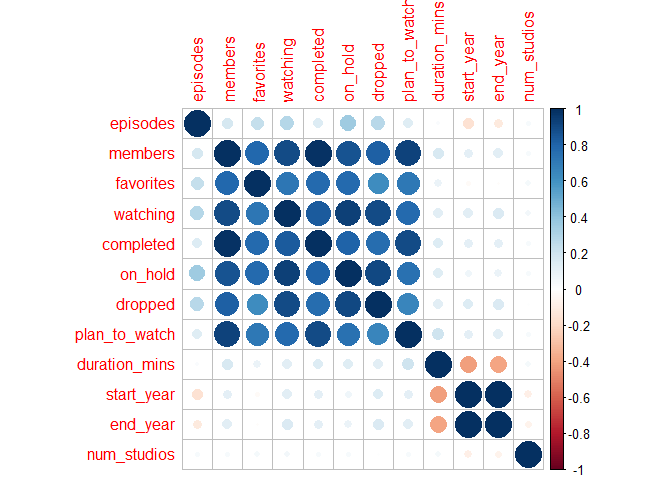
\includegraphics{index_files/figure-latex/unnamed-chunk-12-1.pdf}

Notably, number of members, favorites, watching, completed, on-hold,
dropped, and plan to watch are moderately to highly correlated. In order
to correct for this, we will retain number of community members in each
anime's group as the representation of membership to the anime's fan
base in our dataset. Additionally, start year is highly correlated with
end year so we'll just retain information on start year and instead
create a variable representing number of years running.

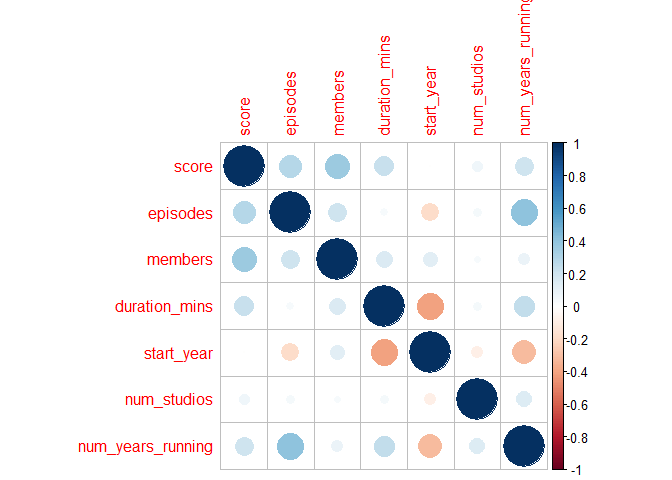
\includegraphics{index_files/figure-latex/unnamed-chunk-14-1.pdf}

After removing the variables strongly correlated with number of
variables, we have a better distribution of variables without unexpected
multicollinearity. We move on to stepwise selection with these
predictors as well as our non-numeric predictors to choose the best
variables to model MyAnimeList score.

To recall, we retain the following variables as the subset of predictors
to choose from: type, number of episodes, primary studio, secondary
studio, source, rating, number of members in that anime's community,
duration in minutes per episode, airing start year, number of animation
studios working on the anime, and binary/indication variables for the
following variables: Action, Adventure, Comedy, Drama, Fantasy,
Historical, Kids, Magic, Mecha, Romance, School, Sci-Fi, Shounen, Slice
of Life, and Supernatural.

In order to validate the generalizability, we will perform stepwise
selection on 80\% of our dataset, which we'll call the training data.
The remaining 20\% will be saved to test the accuracy of our model on.

After going through stepwise selection, we yield the following model:

\begin{center}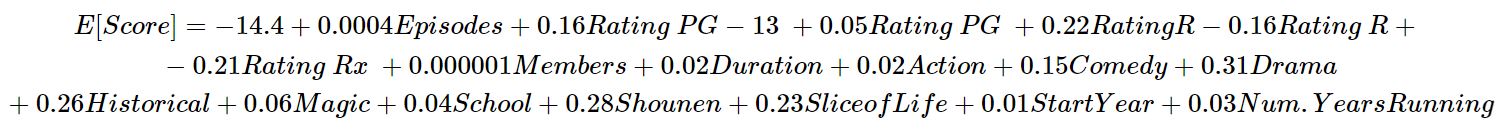
\includegraphics[width=20.81in]{img/mod_equ} \end{center}

where \(E[Score]\) is the expected value of the score of each anime.

\begin{verbatim}
## 
## Call:
## lm(formula = score ~ episodes + rating + members + duration_mins + 
##     action + comedy + drama + historical + magic + school + shounen + 
##     slice_of_life + start_year + num_years_running, data = train)
## 
## Residuals:
##     Min      1Q  Median      3Q     Max 
## -3.5290 -0.3887  0.0254  0.4292  1.8228 
## 
## Coefficients:
##                                        Estimate Std. Error t value Pr(>|t|)    
## (Intercept)                          -1.435e+01  1.973e+00  -7.271 4.10e-13 ***
## episodes                              3.973e-04  1.832e-04   2.169 0.030137 *  
## ratingPG-13 - Teens 13 or older       1.581e-01  3.079e-02   5.134 2.95e-07 ***
## ratingPG - Children                   5.012e-02  4.447e-02   1.127 0.259768    
## ratingR - 17+ (violence & profanity)  2.186e-01  4.212e-02   5.190 2.19e-07 ***
## ratingR+ - Mild Nudity               -1.615e-01  4.207e-02  -3.838 0.000126 ***
## ratingRx - Hentai                    -2.056e-01  4.048e-02  -5.078 3.95e-07 ***
## members                               1.348e-06  5.028e-08  26.804  < 2e-16 ***
## duration_mins                         1.640e-02  1.064e-03  15.421  < 2e-16 ***
## action1                               1.615e-02  2.269e-02   0.712 0.476548    
## comedy1                               1.481e-01  2.062e-02   7.184 7.77e-13 ***
## drama1                                3.114e-01  2.488e-02  12.514  < 2e-16 ***
## historical1                           2.626e-01  3.652e-02   7.190 7.43e-13 ***
## magic1                                6.428e-02  3.200e-02   2.009 0.044598 *  
## school1                               3.519e-02  2.608e-02   1.349 0.177276    
## shounen1                              2.779e-01  2.476e-02  11.224  < 2e-16 ***
## slice_of_life1                        2.273e-01  2.836e-02   8.015 1.36e-15 ***
## start_year                            1.011e-02  9.820e-04  10.298  < 2e-16 ***
## num_years_running                     3.291e-02  9.432e-03   3.489 0.000489 ***
## ---
## Signif. codes:  0 '***' 0.001 '**' 0.01 '*' 0.05 '.' 0.1 ' ' 1
## 
## Residual standard error: 0.6343 on 5078 degrees of freedom
##   (2247 observations deleted due to missingness)
## Multiple R-squared:  0.3634, Adjusted R-squared:  0.3612 
## F-statistic: 161.1 on 18 and 5078 DF,  p-value: < 2.2e-16
\end{verbatim}

So, what does this tell us? A few things actually. Among the anime in
our training data, the more \textbf{episodes} that an anime has, the
more likely it is to be scored highly on MAL. With each new additional
episode in an anime, we expect a 0.0004 increase in score.

In regard to content ratings, we list the rating labels in order of
highest to lowest scored, holding all other variables in our model
constant:

\begin{enumerate}
\def\labelenumi{\arabic{enumi})}
\item
  R - 17+ (violence \& profanity)
\item
  PG-13 - Teens 13 or older
\item
  PG - Children
\item
  G - All Ages
\item
  R+ - Mild Nudity
\item
  Rx - Hentai
\end{enumerate}

Notably, there doesn't seem to be a linear relationship between rating
and score. While generally audiences tend to like content that are on
the maturer side (rated PG-13 and R - 17+), there's a limit to exactly
\emph{how} spicy audiences like their content to be cooked up for them.
Particularly, as we see an upward trend in score from ratings G, PG,
PG-13, and R- 17+, the next too more intense levels of content, R+ for
mild nudity, and Rx for full blown Hentai are in fact scored the lowest
on the list. Meaning, we mature themes seem to be a hit among the MAL
community, but explicit content\ldots{} not so much.

\includegraphics{./img/watch_tv.gif}

As expected, number of members in that anime's MAL group is positively
associated with that anime's score. For every one additional member, we
expect a 0.000001 increase in score, holding all other variables in the
model constant. While this change seems small, it's helpful to keep in
mind the range of values in each anime's group.

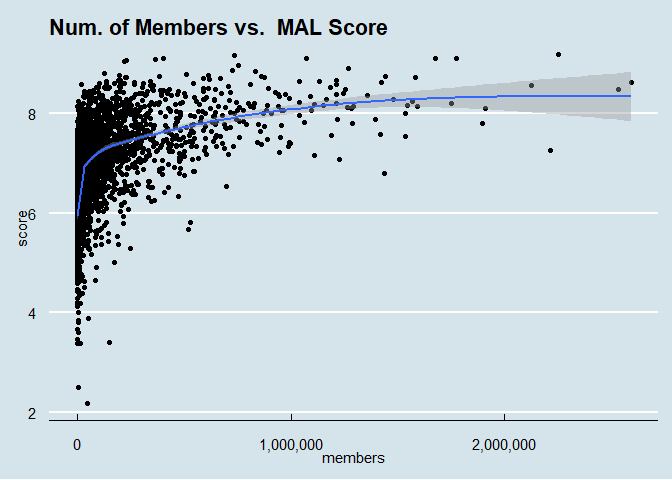
\includegraphics{index_files/figure-latex/unnamed-chunk-19-1.pdf}

In our train dataset, the number of members within each anime's group
ranges from 1 to 2,589,552 with a median value of 4,568 which is a
\emph{huge} range! This means, for example, we expect the score of an
anime with a member base the size of the median value of 4,568 to
increase by an estimated 0.005 (0.000001*4,568 members) points.

Now let's talk duration per episode. Our model shows that there is a
positive association between the number of episodes in a season, and the
score of an anime. The more the merrier, one might say. With each
additional minute per episode, the score is expected to increase by
0.02. Of course, the expectation of duration is different by type
(e.g.~TV, Movie, OVA).

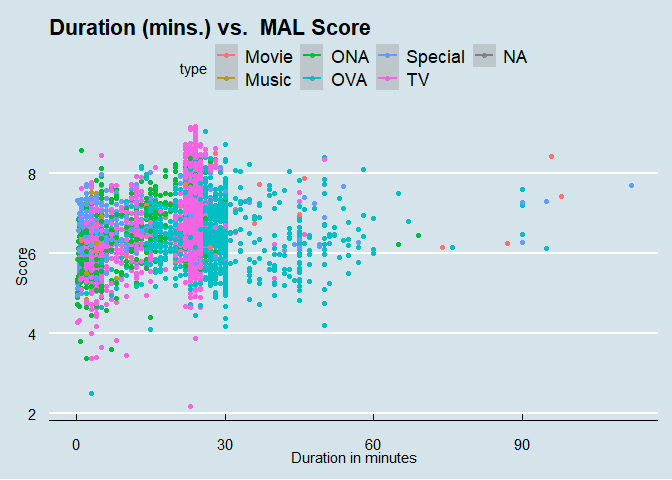
\includegraphics{index_files/figure-latex/unnamed-chunk-22-1.pdf}

Though, there's no hard and fast rules for how long these mediums can
be, we see from the scatterplot above that while anime for TV typically
tend to keep within 30 minutes or less, mediums like OVAs are more
variable in their length (see scatterplot above). Additionally,
specials, music videos, and ONAs tend to be shorter and movies tend to
be longer.

How about genre? Do some genres tend to be more well received than
others, at least in regard to score?

Well, according to our model, these are the genres that are scored from
highest to lowest on MyAnimeList.net in order, holding all other
variables in our model constant:

\begin{enumerate}
\def\labelenumi{\arabic{enumi})}
\item
  Drama
\item
  Historical
\item
  Shounen
\item
  Slice of Life
\item
  Comedy
\item
  Magic
\item
  School
\item
  Action
\end{enumerate}

Now, you may be wondering for example,
\textit{how come action isn't ranked higher on this list?!} I mean, from
My Hero Academia to Jujutsu Kaisen, it's no doubt that action anime
encompass a huge portion of the hits right now. However\ldots{} action
is also the most frequently reported genre in 2020. So while it's a
standout among the hits, in the grand scheme of things, while there are
amazing action anime that are being ranked and perceived well, there are
also action anime out there that are performing less favorably among
crowds. In fact, it seems that the action genre may even be
over-saturated with the good, the bad, and the ugly. In other words,
purely slapping the genre of action on your anime doesn't make it an
automatic hit. Yes, it's true. Audiences won't just froth at the mouth
at characters going toe-to-toe in combat without it having that special
`oomph' to it that really makes it a generational favorite.

\textbf{This just in, newer anime are in!} According to our model, with
each additional year of an anime airing, we expect a score increase of
0.01. Of course, this may just be a consequence of recency bias and how
anime are often more likely to be popular and perceived well in their
prime (i.e.~when they're still airing and fresh off the presses). But
it's interesting to think how year-to-year advancements in animation and
technology may have contributed to the perception of newer anime.

Additionally, we can take into account how many years an anime has been
running. Evidently, anime that have been on-going for longer have
significantly higher scores than those that have not. Perhaps being in
the good graces of key audiences is what have allowed them to persist
for so long. According to our model, with each additional year of run
time, the score value is expected to increase by 0.03.

Now that we've summarized what our model is trying to tell us about the
anime in our training set, we can apply our model to our withheld test
set to see how well it performs on data it hasn't seen!

We'll use mean absolute error (MAE) as our measure of score prediction
error, which is measured as such:

\begin{center}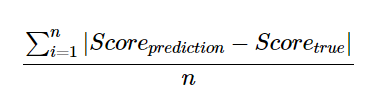
\includegraphics[width=5.42in]{img/mae} \end{center}

We use our model to predict on our test data and collect prediction
error on each observation. The plot below shows that the distribution of
prediction errors seems to roughly normally distributed with a maximum
error observed of 2.64 and a minimum error of -1.79. To put things into
context, on a scale of 1-10, which is the scale of MAL score, an error
of 2.64 can be a gross overestimation of an anime's score. This maximum
value seems to be an outlier though as the majority of prediction errors
hover around 0.

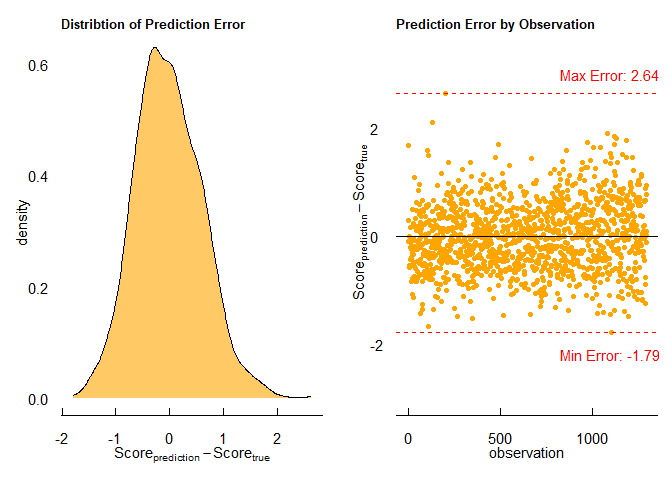
\includegraphics{index_files/figure-latex/unnamed-chunk-28-1.pdf}

And so the mean absolute error is 0.5. So, on average, we can expect a
0.5 (or 1/2 a point) prediction error from this model. With that being
said, it may be reasonable to conclude that our model generally performs
well on our test data and we may have some comfort in the validity of
the inferential conclusions drawn by our model!

\hypertarget{scores-galore-do-users-preemptively-score-anime-does-the-general-consensus-change-from-all-users-to-users-who-have-marked-the-anime-as-completed}{%
\subsubsection{Scores Galore: Do users preemptively score anime? Does
the general consensus change from all users to users who have marked the
anime as
`completed'?}\label{scores-galore-do-users-preemptively-score-anime-does-the-general-consensus-change-from-all-users-to-users-who-have-marked-the-anime-as-completed}}

Alright! We've talked about the key predictors of anime performance and
to what magnitude these factors are expected to affect MAL score. We do
well to recall that MAL score is averaged from scores assigned to anime
from \emph{all} users. A question of interest - does this averaged score
significantly differ from the average score given only by users that
have marked that anime as `completed'? And if so, could this give us
insight that users may preemptively score anime or that users that may
score anime before seeing the whole thing may have held a different
opinion if they had seen the whole thing through? Let's investigate.

Earlier, we were able to left-join information on scores given to anime
by users that have marked those anime as `completed' on MAL.

In order to test this, we may derive a vector of pairwise differences
between the MAL score and the average score given by users that have
indicated that they have completed the respective anime:

Score\textsubscript{MAL} - Score\textsubscript{Completed}

If the scores are not significantly different, we may expect that this
vector of differences follow a normal distribution centered around 0.

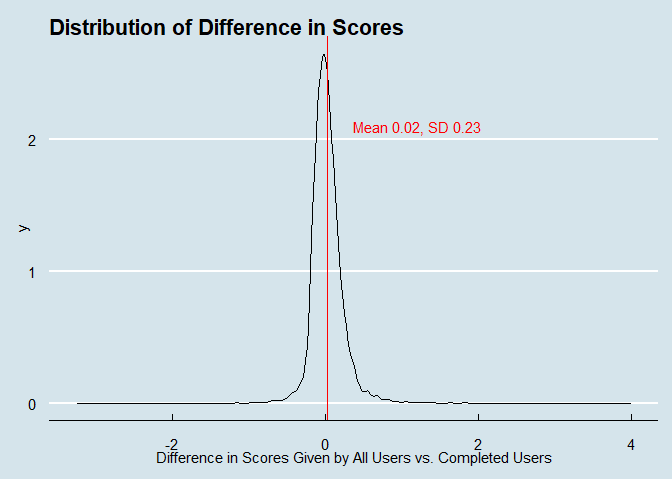
\includegraphics{index_files/figure-latex/unnamed-chunk-31-1.pdf}

The distribution of differences between scores (MAL Score - Completed
Users Score) is centered around a mean of 0.02 with a standard deviation
of 0.23. A mean of 0.02 which is positive, mean that MAL scores
generally tend to be slightly higher than scores given by users who have
marked those anime as completed.

It's difficult to just eyeball this distribution and decide whether or
not the difference between these scores is significantly different or
not. One way to formally test this is by using a \textbf{paired-sample
T-test}. The paired-sample t-test can be used to determine whether the
mean difference between pairs of measurements is 0 or not. Thus, the
following hypotheses are tested:

\begin{center}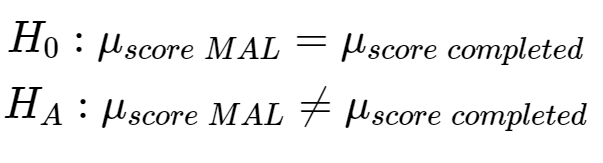
\includegraphics[width=300px]{img/score_t_test} \end{center}

We display the results of the t-test below:

\begin{verbatim}
## 
##  Paired t-test
## 
## data:  anime_full_df$score and anime_full_df$score_comp
## t = 7.8543, df = 6832, p-value = 4.637e-15
## alternative hypothesis: true mean difference is not equal to 0
## 95 percent confidence interval:
##  0.01616230 0.02691326
## sample estimates:
## mean difference 
##      0.02153778
\end{verbatim}

The test yielded a p-value of 4.64 * 10\textsuperscript{-15} which gives
us significant evidence to reject the null hypothesis. Thus, we may
conclude that the mean difference between the sets of scores is not
statistically zero. In particular, it's possible that generally users
are preemptively scoring these anime when they otherwise may have had a
worse opinion of the content had they completed the anime. Though, this
is just a theory as to why we may be seeing a difference between the
scores. We would have to do more extensive research like conducting an
experiment or navigating a causal conclusion in order to explain why
this phenomenon is observed in the data.

\hypertarget{how-long-is-too-long}{%
\subsubsection{How long is too long?}\label{how-long-is-too-long}}

\includegraphics{./img/rampo.gif}

We've all heard the age-old qualm with some anime these days. Though
fans alike love it when our favorite story lines and characters keep
shoveling quality content into our trying lives, when is enough enough?
Die hard fans can all name at least one show where they felt the story
was dragged on and on when really, it would've just been optimal to end
it several episodes or even seasons ago.

So, how long is too long? Is there an optimal range of episodes that an
anime should be in order to leave the audience satisfied?

There are a lot of ways to try and answer this question, but I'm going
to do it by means of regressing number of episodes on anime score.
Recall that score and episodes are both numeric values. Additionally, we
will only consider anime made for TV consumption to keep the anime
relatively within the same playing field in terms of episodic behavior
instead of also including irregular mediums like movies, specials, and
OVAs.

First, we chose to synthesize the number of anime that fall under each
episode count. We arbitrarily decided to retain information on episodes
that at least 5 anime fall under so that no one anime is driving our
inference on episode count.

After filtering for episodes that have at least 5 episodes under its
belt, we get a range of episodes from 3 to 104 episodes.

Thus, we start by averaging MAL score by episode. According to the trend
that we observe, there doesn't seem to be a strong negative or positive
relationship between number of episodes and score. Though, what is
interesting is where we observe a maximum average score.

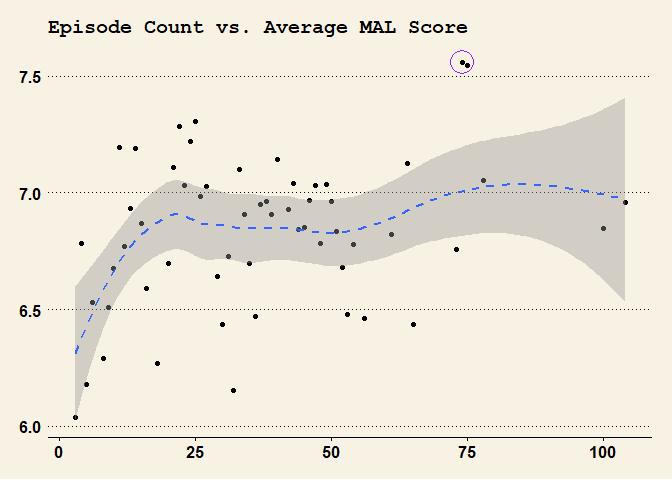
\includegraphics{index_files/figure-latex/unnamed-chunk-36-1.pdf}

We observe that an episode count of 74-75 episodes yielded the highest
MAL scores on average. After 74-75 episodes, the average scores drop
back down to below 7.5.

Though this isn't confirmatory that 74-75 is now the magic number, it
would be useful to see how this range fairs in MAL datasets from other
years as well.

\hypertarget{what-can-synopsis-tell-us-about-score}{%
\subsubsection{What can synopsis tell us about
score?}\label{what-can-synopsis-tell-us-about-score}}

Included in the MyAnimeList database is a synopsis on the anime. Have
you ever wondered, can the synopsis of an anime be a good indicator of
score? What kinds of words often appear in anime that score highly
vs.~those that score lowly?

In order to characterize what it means for an anime to score lowly,
averagely, or highly, we categorize score into ordered categories.
Particularly, we'll be categorizing score into three separate score
categories: low, medium, high. Anime with scores less than 6 were put
into the low category, those with scores greater than or equal to 8 were
placed into the high category, and all other anime were placed into the
medium category.

After categorizing the score variable, we get that only 5.6\% of anime
fall into the high category on MAL, 18\% of anime fall into the low
category, and the remaining 76.4\% of anime fall into the medium
category.

We collect the synopses from this anime belonging to each score group
(low, medium, high) and concatenate/collapse them together.

In order to get meaningful analyses, we will remove stop words from the
\href{http://snowball.tartarus.org/algorithms/english/stop.txt}{Snowball
stop word list}. We'll also add the words `source' and `ann' to the stop
words list because they aren't of contextual significance and often
appear in MAL synopses. We check the frequency of the words that appear
within synopses of lowly scored, medium scored, to highly scored anime
on MAL. We retain information on the top 20 most frequent words that
appear in each categorization of score. In order to scope out the most
meaningful words, we will remove words that appear in all three of the
20 list for anime rated low, medium, and high. These words were one,
world, school, new, life, however, high, two, can, day, time, now,
young.

And so we're left with the following information -

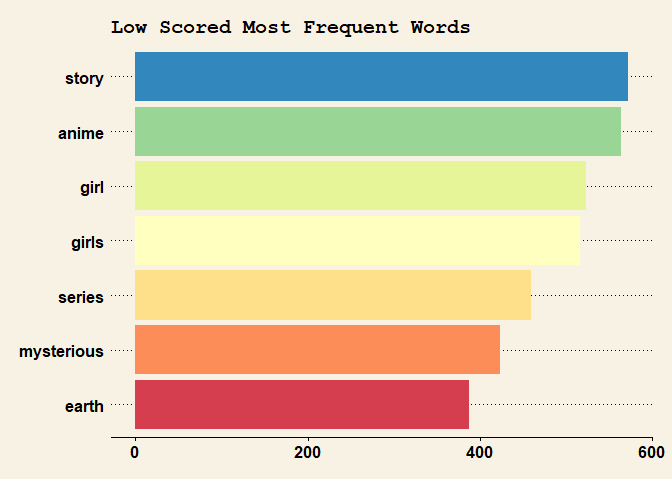
\includegraphics{index_files/figure-latex/unnamed-chunk-44-1.pdf}
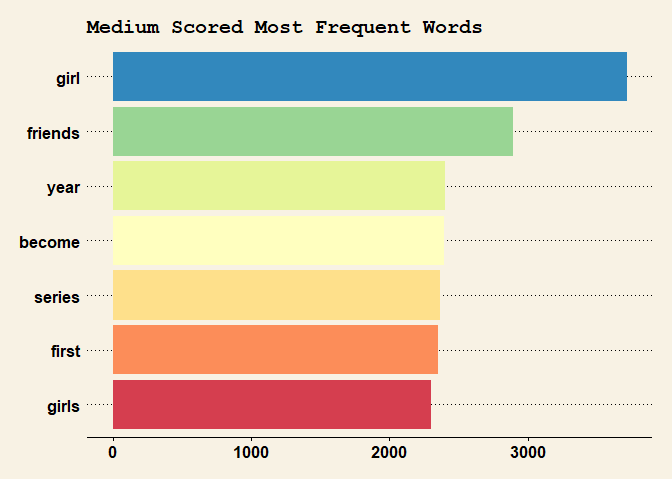
\includegraphics{index_files/figure-latex/unnamed-chunk-44-2.pdf}
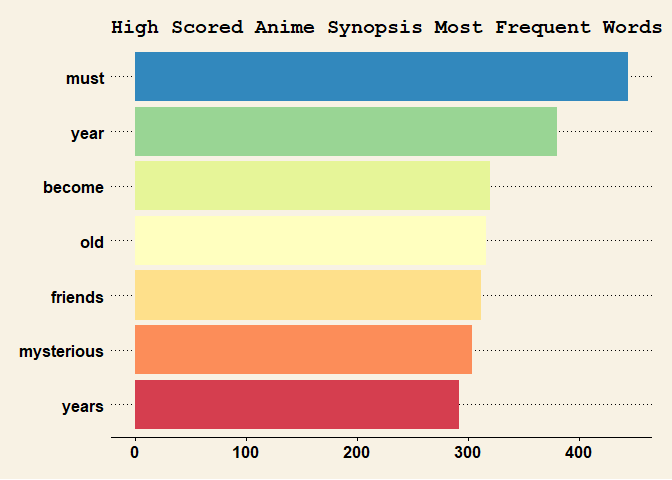
\includegraphics{index_files/figure-latex/unnamed-chunk-44-3.pdf}

A few things of note, anime involving a \texttt{girl} or \texttt{girls}
tend to be more popular as these words appear most frequently for medium
and highly scored anime synopses but not in lowly scored anime. Anime
involving \texttt{friends} can be found in both highly scored anime and
lowly scored anime so it seems the power of friendship is not too
polarizing one way or the other. The same thing goes for the words
\texttt{year} and \texttt{become}. Interestingly, \texttt{must}, and
\texttt{old} standout within anime lowly scored. Just a few of many
observations to take away from this exercise.

For next steps, we can look into adjusting for the number of words in
each synopsis or even extending our synopsis analysis into sentiment
analysis.

\hypertarget{so-what-did-we-learn}{%
\subsection{So what did we learn?}\label{so-what-did-we-learn}}

\end{document}
